% !TeX TS-program = txs:///duck
\documentclass{standalone}

\usepackage{tikzlings}
\usepackage{tikzducks}

\begin{document}

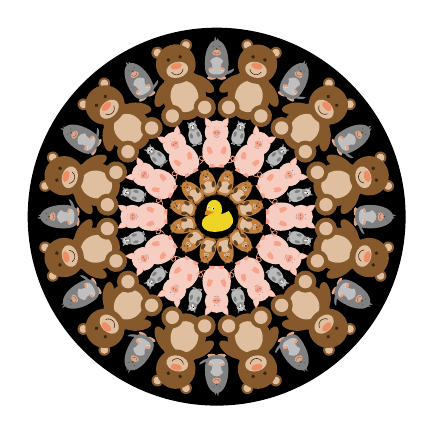
\begin{tikzpicture}
\fill[black] (0,0) circle (2.4);
\foreach \x in {0,30,...,360}{
%\koala[rotate=\x,yshift=60]
\moles[rotate=\x,scale=0.25,yshift=195]
\bear[rotate=\x+15,scale=0.5,yshift=70]
\pig[rotate=\x,scale=0.3,yshift=55]
\rhino[rotate=\x+15,scale=0.15,yshift=175]
\marmot[rotate=\x+15,scale=0.17,yshift=42]
}
\duck[scale=0.2,xshift=-30,yshift=-30]
\end{tikzpicture}

\end{document}}as
